\documentclass[10pt,twocolumn,letterpaper]{article}

\usepackage{statcourse}
\usepackage{times}
\usepackage{epsfig}
\usepackage{graphicx}
\usepackage{amsmath}
\usepackage{amssymb}
\usepackage{enumitem}
\usepackage[hyphens]{url}
% Include other packages here, before hyperref.

% If you comment hyperref and then uncomment it, you should delete
% egpaper.aux before re-running latex.  (Or just hit 'q' on the first latex
% run, let it finish, and you should be clear).
\usepackage[breaklinks=true,bookmarks=false]{hyperref}

\statcoursefinalcopy



\setcounter{page}{1}
\begin{document}


%%%%%%%%%%%%%%%%%%%%%%%%%%%%%%%%%%%%%%%%%%%%%%%%%%%%%%%%%%%%%%%
% DO NOT EDIT ANYTHING ABOVE THIS LINE
% EXCEPT IF YOU LIKE TO USE ADDITIONAL PACKAGES
%%%%%%%%%%%%%%%%%%%%%%%%%%%%%%%%%%%%%%%%%%%%%%%%%%%%%%%%%%%%%%%



%%%%%%%%% TITLE
\title{Hate Speech Detection with Deep Learning Models in PyTorch}


\author{Carlos Eduardo Posada\\
{\tt\small c.posada@mpp.hertie-school.org}
\and
Maximilian Kupi\thanks{These authors will be sharing the project between the NLP and Python class.}\\
{\tt\small m.kupi@mpp.hertie-school.org}
\and 
Michael Bodnar\\
{\tt\small m.bodnar@mpp.hertie-school.org}
\and
Nikolas Schmidt\footnotemark[1]\\
{\tt\small n.schmidt@mpp.hertie-school.org}}



\maketitle
%\thispagestyle{empty}


% MAIN ARTICLE GOES BELOW
%%%%%%%%%%%%%%%%%%%%%%%%%%%%%%%%%%%%%%%%%%%%%%%%%%%%%%%%%%%%%%%

%%%%%%%%% BODY TEXT
\section{Introduction}
This project aims to develop and implement a tool that identifies hate speech on social media. We plan to apply a two-sided hybrid natural language deep learning approach to classify data retrieved from Twitter.

\begin{figure}[h]
    \begin{center}
        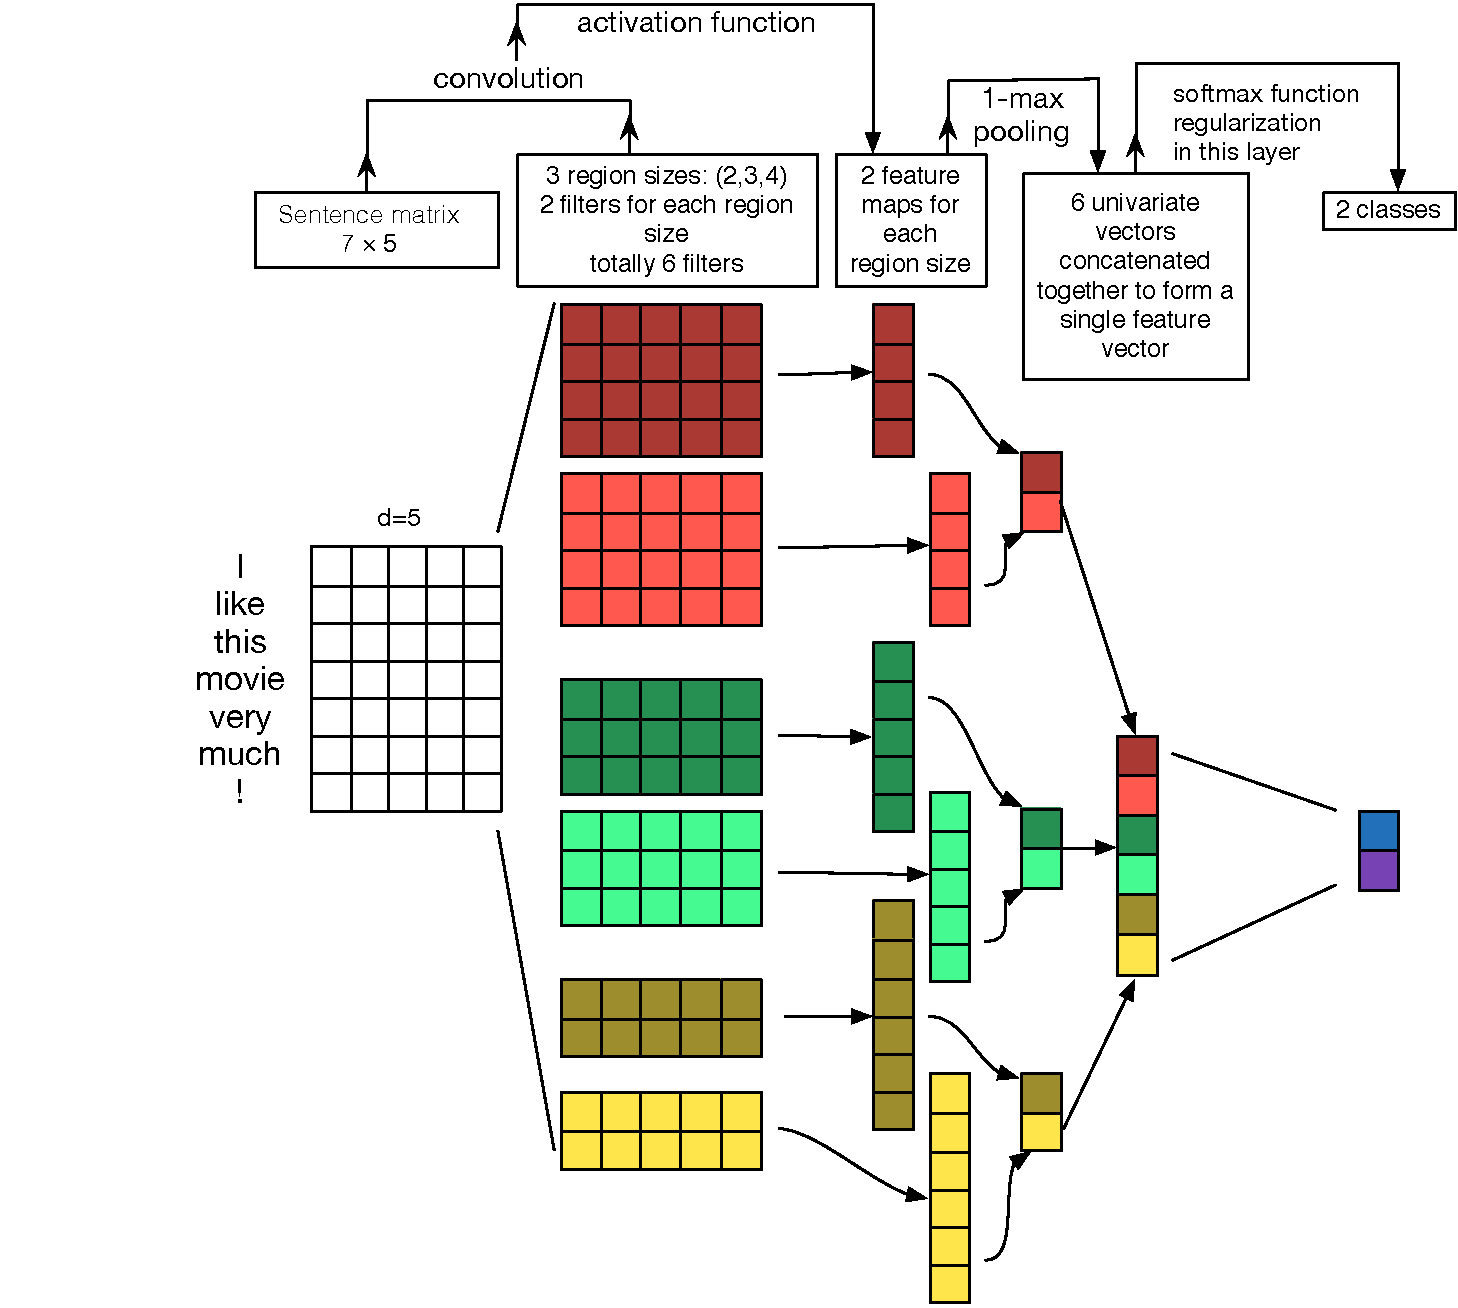
\includegraphics[trim={3.5cm 0 0 0},scale=0.4]{figures/CNN.pdf}
        \caption{Example illustration of a Convolutional Neural Network architecture for sentence classification \cite{Zhang2015}}
        \label{Fig:CNN}
    \end{center}
\end{figure}

Firstly, we plan to apply two different data pre-processing methods to obtain two input matrices: 
\begin{enumerate}[label=(\alph*)]
    \item transforming technique to create word embedded data from two pre-existing datasets of tweets
    \item dictionary approach to count hateful terms from a database
\end{enumerate}{}

Secondly, we plan to employ a convolutional neural network (see Figure~\ref{Fig:CNN}) in order to classify hate speech based on the two input matrices.\par

The literature on hate speech detection has evolved over the past years, regarding its definition, its context of occurrence, and the applied computational methods. In its beginnings, surface feature extractions of the text (e.g. token and character n-grams) were combined with other methods (e.g. bag of words, word generalisation or term frequency-inverse document frequency) for classification \cite{Schmidt2017}.\par 

Before neural networks, a number of machine learning algorithms were employed in the literature, for example support vector machines. However, in recent years, neural networks have become the state of the art – in particular in combination with the use of different word-embedding techniques to represent and group text data in a vector space.\par

Research has also explored the utilization of further characteristics of hate speech: Sentiment analysis can work as a sub-approach to hate speech detection, which focuses on strong negative sentiments to differentiate normal from hate speech \cite{Schmidt2017}. However, this has not improved results substantially, in particular when considering the legally-binding definitions of hate speech. For this reason, we plan to use lexical resources with defined hate terms.\par

The next section is going to delve deeper into the motivation to automatically detect hate speech. Section 3 will introduce the methods we plan to use for evaluating our model, while the following section will introduce the datasets and computational setup. The proposal will conclude with detailing the project's modules and each individual team member's contribution thereto.\par

\section{Motivation}

With the widespread use of social media, there are growing concerns about hateful content. Abusive content, such as tweets and Facebook comments, target individuals or particular groups based on ethnicity, nationality, gender identity, sexual orientation or disabilities. Studies have shown that social media can serve as a propagation mechanism and suggested hateful online messages to be predictors of real-world hate crimes \cite{Muller2017}.\par

In order to discourage violence, social networks and other online venues have sought to filter these harmful messages from their platforms. However, manual removal of hateful comments is unfeasible due to the high volume of comments in a growing number of social media venues. Thus, most recently, automatic methods have been employed. As explained in the previous section, detecting, classifying and removing hate speech is a complex task from a technical point of view.\par

Some of the difficulties of these methods include \cite{MacAvaney2019}:
\begin{itemize}
    \item The lack of a common definition of hate speech, which leads to different databases of hateful comments built with different classification criteria. Hate speech detection tools which are trained on these databases can thus carry biases.
    \item The nuances of natural language, such as sarcasm, sentiment and double meanings, increase the difficulty of discerning between hate speech and allowed free expression.
    \item Keeping up with the lexical evolution of hate speech leads to a need to constantly update the datasets.
\end{itemize}\par

Given these difficulties, the use of deep learning methods can bring significant improvements in hate speech detection. For this reason, in a context of high polarization, rising social tensions, and potential deadly consequences of hate speech, we find this project to be particularly relevant.\par

\section{Evaluation}

%What would the successful outcome of your project look like? In other words, under which circumstances would you consider your project to be ?successful??

We will split the data into
\begin{enumerate}
    \item Training dataset (70\%),
    \item Validation dataset (15\%), and lastly,
    \item Testing dataset (15\%)
\end{enumerate}

in order to train and test the model on current standards.

Furthermore, we will use two different measures to compare the quality of different approaches and to judge the overall quality of our model:

\begin{enumerate}
    \item Accuracy
    \item F1-score
\end{enumerate}

Our model will have three different categories that were already labelled in the datasets. We can calculate the accuracy in each category by comparing the output of the model to the labels. The total distribution of the model output will be compared to the total distribution of the gold standard labels.

We will use the $F1$ score for the hate speech category to compare our different approaches. The $F1$ score is a weighted average of \textit{precision} and \textit{recall}.

$$ F1=2*\frac{Precision*Recall}{Precision+Recall}=\left(\frac{2}{\frac{1}{Precision}+\frac{1}{Recall}}\right) $$

\textit{Precision} is the ratio between correctly identified hate speech entries ($TP$, true positive) and overall identified hate speech entries ($TP+FP$, true positive and false positive).

$$ Precision=\frac{TP}{TP+FP} $$

\textit{Recall} is the ratio between true positives ($TP$) and the sum true positives and false negatives ($FN$), i.e. hate speech mistakenly identified as not hate speech \cite{Nottelmann2005}.

$$ Recall=\frac{TP}{TP+FN} $$

\par

\section{Resources}

%What resources are you going to use (datasets, computer hardware, computational tools, etc.)?

The following datasets will be used in the project:
\begin{enumerate}
    \item The "Automated Hate Speech Detection and the Problem of Offensive Language" dataset from Davidson et al. \cite{hateoffensive}, comprised of 25,000 tweets
    \item The "Hate and Abusive Speech on Twitter" dataset from Founta et al. \cite{founta2018large}, comprised of 100,000 tweets
\end{enumerate}

Both datasets have the following respective categories, according to which the data is labelled:

\begin{enumerate}
    \item hate\_speech, offensive\_language, neither
    \item hateful, abusive, normal, spam
\end{enumerate}

In order to merge both datasets, will filter the spam category in the second dataset.\par

Our computing setup (see Figure~\ref{fig:setup} on next page) includes AWS resources which will be deployed through AWS SageMaker. We will use Visual Studio Code and Google Colab to program and preliminary test our model. The training of the model will happen on the remote AWS resources. We will use a GitHub repository~\footnote{\url{https://github.com/MaximilianKupi/nlp-project}.} to exchange the code between these instances as well as to document the project.

\begin{figure}[t]
    \begin{center}
        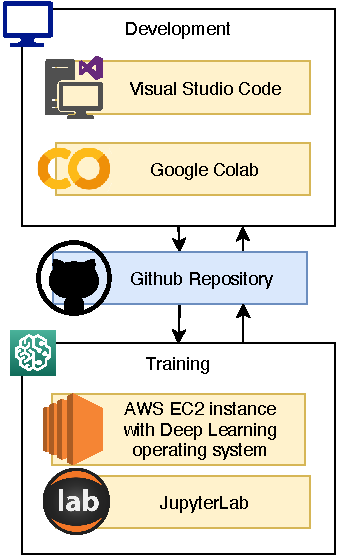
\includegraphics{figures/setup.pdf}
        \caption{Deployment pipeline including IDE for experimentation and AWS resources for training}
        \label{fig:setup}
    \end{center}
\end{figure}
\par


\section{Contributions}
%You are expected to share the workload evenly, and every group member is expected to participate in both the experiments and writing. (As a group, you only need to submit one proposal and one report, though. So you need to work together and coordinate your efforts.)
%Clearly indicate what computational and writing task each member of your group will be participating in.
We split the model design and implementation into two modules and their respective sub-tasks. For each module we assigned a primarily responsible sub-team (in parentheses):\footnote{We have formed the sub-teams such that each sub-team consists of one team member attending both the NLP and the Python class. This person will be the "lead coder" in the sub-team.}
\begin{enumerate}
    \item Data pre-processing and loading \newline(E. Posada \& M. Kupi)
    \begin{enumerate}
        \item Obtaining and cleaning the datasets
        \item Twitter specific text pre-processing
        \item Word / sentence vectorisation (as first data input)
        \item Implementing a dictionary approach potentially based on  \href{https://hatebase.org/}{Hatebase.org} (as second data input)
        \item Splitting data into test, validation and testing set
        \item Specifying and implementing the data loader
        \item Testing and iterating the module  
        \item Creating module-specific visualisations for the final paper
    \end{enumerate}
    \vspace{2cm}
    \item Model architecture and training \newline(M. Bodnar \& N. Schmidt)
     \begin{enumerate}
        \item Choosing width and depth of the model
        \item Choosing optimizer as well as activation and loss functions
        \item Choosing stopping rule, regularisation, dropout, learning rates etc.
        \item Potentially performing a hyperparameter grid search
        \item Running and tracking the training
        \item Training and tuning the model based on the results of the validation set
        \item Creating module-specific visualisations for the final paper
    \end{enumerate}
\end{enumerate}\par 
The paper writing will be divided according to the technical tasks performed by each of the team members. All creative ideation takes place in the whole team. Project management as well as facilitation of the working sessions is done by M. Kupi.\par 

{\small
\bibliographystyle{ieee}
\bibliography{writing/references.bib}
}

\end{document}
